\begin{adjustbox}{width=.95\paperwidth, center}
	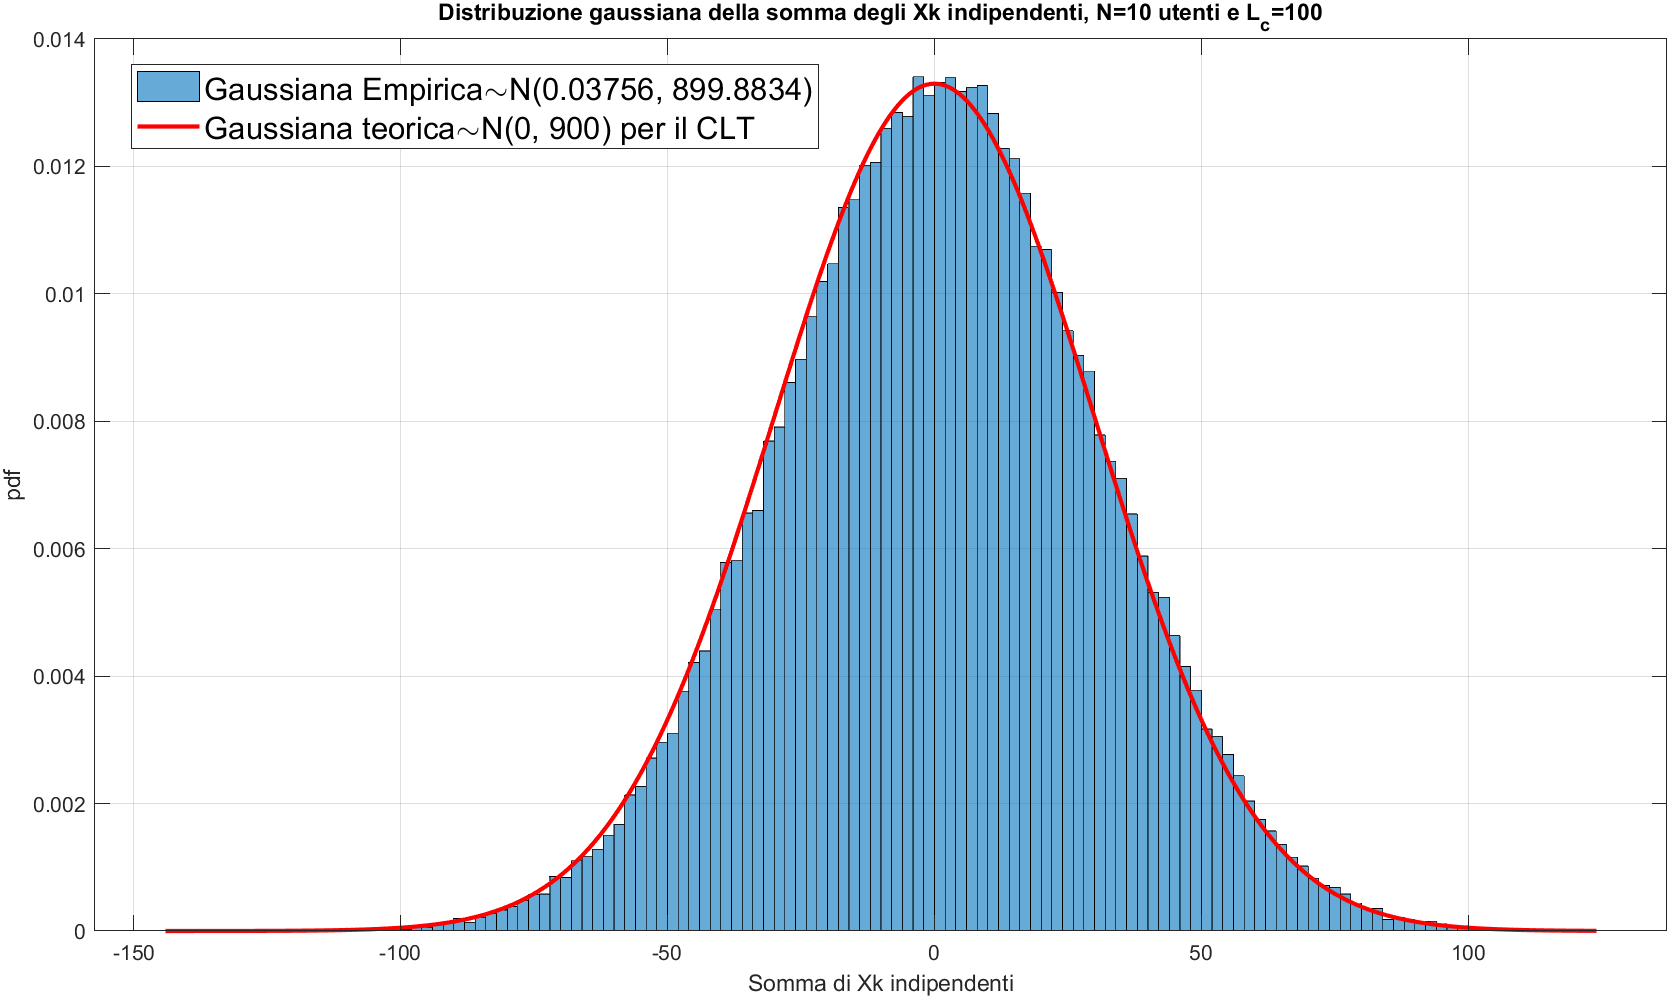
\includegraphics{images/distribuzioneGaussianaEmpTh.png}
\end{adjustbox}\\\\
Svolgendo l'esperimento \( \sum_{k=1}^{L_c}\left(\sum_{n=2}^{N}c_{1k}\cdot c_{nk}\right)
= \sum_{k=1}^{L_c}X_k \) con \(N=10\) utenti e \(L_c=100\) lunghezza del chirping code per ogni utente, si dimostra empiricamente che la somma degli \(X_k\) indipendenti \( \sum_{k=1}^{L_c}X_k = n \) ha una distriuzione gaussiana (di colore blu nel grafico) che segue quella teorica (di colore rosso nel grafico), con media \(0.038 \to 0\) e varianza \(899.883 \to 900=L_c(N-1)\), come era stato dimostrato teoricamente nella pagina precedente.